%%%%%%%%%%%%%%
%%  Template for latex documents
%%  Author: Marco A. Aquino-Lopez
%%  Nota: to get a word document use pandoc
%%  pandoc -f latex Articulo.tex -o Articulo.docx --bibliography=bibliography.bib
%%%%%%%%%%%%%%%%%
%\documentclass [twocolumn,10pt] {article}
\documentclass [10pt] {article}

\usepackage [utf8] {inputenc}
\usepackage[english]{babel}

\usepackage {graphicx}
%\usepackage {amsfonts,unicode-math}
\usepackage {amsthm}
\usepackage {amsmath}
\usepackage {natbib}

\usepackage{hyperref}
\usepackage[in]{fullpage} %To have more in the page
%.____         ___________    ____  ___ 
%|    |   _____\__    _______ \   \/  / 
%|    |   \__  \ |    |_/ __ \ \     /  
%|    |___ / __ \|    |\  ___/ /     \  
%|_______ (____  |____| \___  /___/\  \ 
%        \/    \/           \/      \_/ 

\graphicspath{{Figures/}} %Setting the graphicspath

%Extra packages2
\usepackage{placeins}

%%%%%%

\date{\today}
\usepackage{color}

%%%% To mark notes or added text by Author1 (a1)
%%%% This allows to add notes
%\newcommand{\a1}{\color{red} }  %% begin
%\newcommand{\1a}{ \color{black}} %% end
%\newcommand{\cuta1}[1]{\ac [cut] \ca} %% to mark cut text
%\newcommand{\notea1}[1]{\textcolor{red}{(note)}\footnote{\ac #1 \ca}}  %% To add a note or comment

% %%%% To mark notes or added text by Andres (ac)
 \newcommand{\ac}{\color{red} }  %% begin
 \newcommand{\ca}{\color{black}} %% end
 \newcommand{\cutac}[1]{\ac [cut] \ca} %% to mark cut text
 \newcommand{\noteac}[1]{\textcolor{red}{(note)}\footnote{\ac #1 \ca}}  %% To add a note or comment

% %%%% To mark notes or added text by Marco (ma)
% \newcommand{\ma}{\color{blue} }  %% begin
% \newcommand{\am}{\color{black}} %% end
% \newcommand{\cutma}[1]{\ac [cut] \ca} %% to mark cut text
% \newcommand{\noteam}[1]{\textcolor{red}{(note)}\footnote{\ac #1 \ca}}  %% To add a note or comment


% NOTE: To produce blinded version, replace "0" with "1" below.
\newcommand{\blind}{1}
\newcommand{\papertitle}{
	Decoding Peatland Dynamics: A Bayesian Model for Inferring System Shifts and Carbon Decomposition
}

\begin{document}
	\def\spacingset#1{\renewcommand{\baselinestretch}%
		{#1}\small\normalsize} \spacingset{1}
	%%%%%%%%%%%%%%%%%%%%%%%%%%%%%%%%%%%%%%%%%%%%%%%%%%%%%%%%%%%%%%%%%%%%%%%%%%%%%%
	\if1\blind
	{
		\title{\textbf{\papertitle}}

		\author{Marco A Aquino-L\'opez\thanks{
				Department of Geography, University of Cambridge, 
				Cambridge, United Kingdom
				email: \texttt{aquino@cimat.mx} } \thanks{Corresponding author.}
					\and
			Jingjing Sun\thanks{
				Northeast Normal University
				China. 
				email: \texttt{sunjj878@nenu.edu.cn}}
					\and
			Angela Gallego-Sala \thanks{
				Department of Geography, Exeter University,
				Exeter, United Kingdom.
				email: \texttt{a.gallego-sala@exeter.ac.uk}  }
			}
		\maketitle
	} \fi

	\if0\blind
	{
		\bigskip
		\bigskip
		\bigskip
		\begin{center}
			{\LARGE\bf \papertitle}
		\end{center}
		\medskip
	} \fi
\bigskip

\begin{abstract}
	This paper introduces a novel Bayesian model designed to provide a sophisticated understanding of carbon dynamics within peatland ecosystems. Our model takes inspiration from the classic Clymo model, while addressing some limitations of the traditional approach. Specifically, the new model allows for the variable influxes of carbon, even in the deepest sediment layers, offering a more realistic and nuanced portrayal of carbon behaviour in peatlands. 


We introduce a novel aspect: a weighted function that is instrumental in defining a boundary between two distinct systems within the peatland, but also allows for a smooth transition from one system to another. This feature is particularly relevant in scenarios where a shift in the water table leads to a significant difference in decomposition rates above and below the water line.

	Our model embraces the complexity of peatlands and underscores the importance of Bayesian statistics for making accurate inferences about system shifts and carbon decomposition in these vital ecosystems. The paper further elaborates on the theoretical underpinnings of the model, its application, and the implications of our findings for peatland management and carbon cycle science. With this work, we aim to provide a robust tool for advancing research on peatland dynamics and their role in the global carbon cycle. 

\end{abstract}
	\noindent%
	{\it Keywords:} Clymo model, carbon accumulation, Bayesian statistics	\vfill
	\newpage
	\spacingset{1.45} % DON'T change the spacing!

\section{Introduction}
Peatlands play a crucial role in the global carbon cycle, acting as significant carbon sinks that help mitigate the impacts of climate change. Understanding the intricate dynamics of carbon influx and decomposition in these ecosystems is paramount for developing effective strategies for their management and conservation. However, carbon dynamics in peatlands can be complex, affected by myriad variables and processes occurring at different layers of the ecosystem.

Traditional models, such as the Clymo model, have provided valuable insights into these dynamics, but they often fall short in capturing the variable nature of carbon influxes, particularly in the deepest parts of peatland sediments. Furthermore, these models typically delineate sharp boundaries between different systems within peatlands, neglecting the gradual transitions that often occur in reality.

In response to these limitations, this paper introduces a novel Bayesian model for inferring system shifts and carbon decomposition in peatlands. This model is built upon the foundations of the Clymo model but extends its capabilities by incorporating a weighted function to allow for a smooth transition between different systems. This is especially relevant when considering phenomena like changes in the water table, which can drastically alter the decomposition rates above and below the water line.

The remainder of this paper is organized into four chapters, each focusing on a key aspect of our research: Chapter 2 delves into the specifics of the data utilized for this study and discusses the problems and limitations associated with conventional peatland carbon models, and the need for an improved, more nuanced approach. Chapter 3 details the development and structure of the Bayesian model. It presents the mathematical and theoretical foundations of the model, and outlines the innovative use of a weighted function to infer system transitions in peatland ecosystems. Chapter 4 provides a comparative analysis of our model's performance relative to traditional models. We demonstrate the enhanced capabilities of our model, particularly in modelling variable carbon influxes and smooth system transitions. Chapter 5 summarizes the findings of our study and discusses their implications for peatland management and carbon cycle research. 


\section{Carbon estimation: Data and Problems}

\section{Model Construction}



\subsection{Logistic Regression for Transition dynamics}
The transition between two distinct environments within a peat core is of significant interest in geological and environmental research. This text elucidates the use of a logistic function to accurately represent this transition. The logistic function, characterized by two parameters - alpha and delay, effectively describes the depth at which the transition occurs. By providing a mathematical explanation of the logistic function and its parameters, this text aims to enhance the understanding and application of this modelling approach for analysing peat core data.

\begin{eqnarray}
	w(x) =\frac{ 1} {1 + \exp(-k(x - \nu))}, \label{eq:logit}
\end{eqnarray} 
equation \ref{eq:logit} is logistic function, where $k$ represents the grow of the function and $\nu$ represents the depth at which the logistic function equals $.5$, i.e. the mid-point of transition between the two environments. In order to obtain a more meaning parameter, we redefine parameter $k$. $\nu$ represents the mid-point of the transition which meaning is clear in the context of the peatland, it is the mid-place of the transition between environments, on the other hand $k$ represents the grow rate of the function but environmental sciences are more interested in the length on which this transition take place. For this we refine the parameter as follow. We first define a tolerance value, $\epsilon>0$, such that we consider that when $w(x_i)=\epsilon$ is the moment when the transition from which the environment shift begins. Now because we are interested in the distance that it takes the transition we define $x_1$ as the depth at which the transition begins so half of this transition can be define as $\gamma = (\nu-x_1)$, if we also define $\epsilon' = \log(\frac{\epsilon}{1-\epsilon})$. Now we can rewrite \ref{eq:logit} as:
\begin{eqnarray}
	w(x) =\frac{1}{1 + \exp\left(\frac{\epsilon'}{\gamma}(x - \nu)\right)}. \label{eq:w_fun}
\end{eqnarray} 

Equation \ref{eq:w_fun} provide us a function to describe the transition from one environment to another where $\nu$ represents the midpoint of this transition. This value is equivalent to the A/C boundary describe by [citar el articulo donde se hace el AC boundery]. On the other hand we this function allows for a smooth transition from one environment to the other one where $\gamma$ described the length of this transition. 
For our implementation we define $\epsilon=0.001$, using this value figure \ref{fig:w_function} shows an example of this transition function, In this example $\nu=50$ and $\gamma = 20$. This results in a transition which begins at depth 30 and end at depth 70. This means that material which is above 30 cm and below 70 cm accumulates and decays according to a single model. For material which lies in between this period, within the interval of 30 and 70 cm the material decomposes according to two distinct model and each sample is affected by each model according to the transition function, material which lies between 30 and 50 cm (between $(\nu-\gamma, \nu)$) are more affected by the model describing surface level decomposition, and oposite for material in the interval $(\nu,\nu +\gamma)$.


NOTA: cambiar el nombre de weighted function a transition function


\begin{figure}[!]
	\begin{centering}
		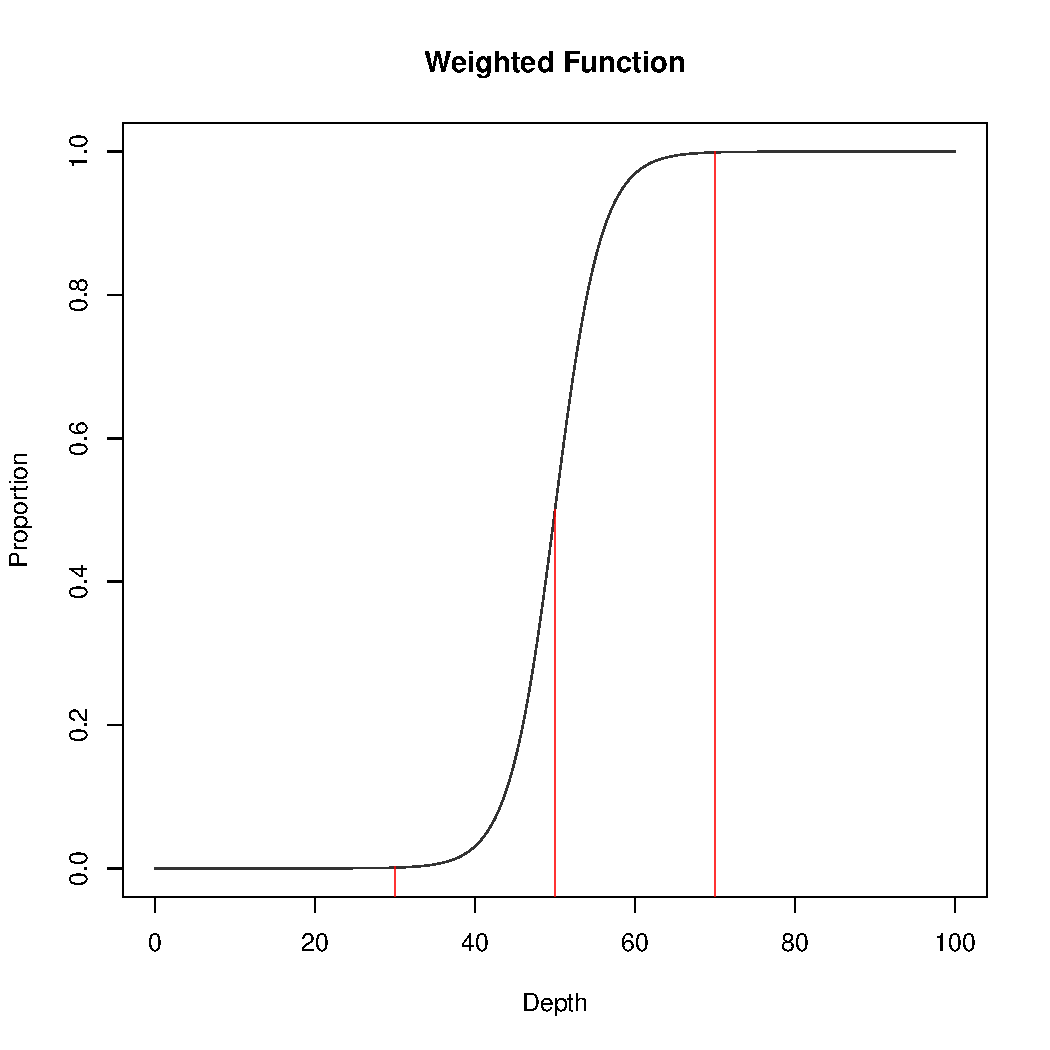
\includegraphics{weighted_fun.pdf}
		\caption{Representation of the weighted function with a boundary at depth 50 and 20 cm of delay.}
		\label{fig:w_function}
	\end{centering}
\end{figure}

It is important to note that this transition function depends only in two parameters ($\nu$ and $\gamma$). Together with the parameters described the previous section which rule the decomposition and influx of the material we can put this model into a Bayesian framework which will allow us to infer all the parameters of the model

\subsection{Likelihood}

It is important to note that the bulk density is estimated at samples of interval ($x-\delta,x$). Using the decomposition model presented preciously we can assume that each measurement of bulk density can be define as follows:

\begin{eqnarray}
	b_i\mid \alpha_a,\alpha_b, \beta_a,\beta_b,\gamma, \nu \sim \mathcal{N}\left( w(x_i,\nu,\gamma) \mathcal{F}(t(x_i),\alpha_a,\beta_a) + (1-w(x_i,\nu,\gamma)) \mathcal{F}(t(x_i),\alpha_b,\beta_b)          ,b_i \cdot \phi  \right), \label{eq:normal}
\end{eqnarray} 
where $\mathcal{F}(t(x_i),\alpha_a,\beta_a) $ is the decay model at affecting the top part of the sediment (see equation []), $\mathcal{F}(t(x_i),\alpha_b,\beta_b)$ the decay model affecting the bottom part of the sediment and $\phi$ is a error measurement multiplier, for our model we will define it as $\phi=.01$ which means the standard deviation is about $1\%$ of the measuring material, this value is usually define by the laboratory and there is no reason to assume it to be random. With equation \ref{eq:normal} we can now define the likelihood as:
\begin{eqnarray}
	\mathcal{L}(\alpha_a,\alpha_b, \beta_a,\beta_b,\gamma, \nu) = \prod_{i=1}^n\frac{1}{2\pi b_i\cdot\phi} \exp\left(-\frac{( w(x_i,\nu,\gamma) \matcal{F}(t(x_i),\alpha_a,\beta_a) + (1-w(x_i,\nu,\gamma)) \mathcal{F}(t(x_i),\alpha_b,\beta_b) - b_i)^2 }{ 2( b_i \cdot \phi )^2 }  \right), \label{eq:normal}
\end{eqnarray} 


\subsection{Decomposition Model}

Peatlands are complicated system with many different model created to infer the decomposition dynamics. In our approach, we will use the some what simple approach mentioned by \citet{Clymo1984}. If we make the same assumption which is that the rate of accumulation of dry matter to the sediment column at any age, $m(t(x))$, is by the rate of addition $m_0$. Let $\alpha_a$ be the decay of the organic material so this model can be define by:
\begin{eqnarray}
	\frac{dm(t(x))}{dt(x)} = m_0 - \alpha_a m(t(x))
\end{eqnarray}
This differential equation has an explicit solution by we have the initial condition as $t(0)=0$, $m(0)=0$. The solution is given by,
\begin{eqnarray}
	m(t(x)) = \frac{m_0}{\alpha_a} \left( 1- e^{-\alpha_a t(x)}   \right)	
\end{eqnarray}

Note that solution is possible if 



\section{Comparison}







\section{Conclusion and Discussion}












\bibliographystyle{apalike}
\bibliography{bibliography.bib}
\newpage


\end{document}

